\documentclass[12pt,a4paper]{article}
%\usepackage[utf8]{inputenc}
\usepackage[margin=0.5in]{geometry}
\usepackage{graphicx}
\author{
  Drew, Keith\\
  \texttt{keithd@vandals.uidaho.edu}
  \and
  Jaszkowiak, Tyler\\
  \texttt{jasz7989@vandals.uidaho.edu}
  \and
  Pearhill, Gabe\\
  \texttt{pear9915@vandals.uidaho.edu}
  \and
  Klingenberg, David\\
  \texttt{bigwookie@gmail.com}
  \and 
  Fuhrman, Wayne\\
  \texttt{fuhr0438@vandals.uidaho.edu}
  \and
  Goes, Chris\\
  \texttt{goes8945@vandals.uidaho.edu}
}
\title{Diagram Assembly Document}
\begin{document}
\maketitle
\section{Dictionary}
\begin{itemize}
\item Board: The game board, this holds nearly all visual information about the game and state. The class holds random event flags, which will become more specific, that indicate global events.
\item Province: A province is a group of hexes that are related by controlling faction. Essentially like the United States of Hexes. 
\item Hex: A discrete location on the board. Hexes are represented by a unique ID, terrain, and a stack of units that can be empty.
\item Stack: A collection of units and characters, bound by the rules of the game. Ie, 0 or more characters, and 0-2 units. Also, special considerations for movement phase, flying units, and monsters.
<<<<<<< HEAD
\item Vortex: A vortex is a movable unit, from the system's point of view. A character can control vortices under certain conditions. Otherwise movement, creation, and destruction of vortices is automated.
=======
\item Vortex: A vortex is a moveable unit, from the system's point of view. A character can control vortices under certain conditions. Otherwise movement, creation, and destruction of vortices is automated.
>>>>>>> 521092394ab6230c68dbf71a0ed7ddbd74776aa2
\item Diplomacy: An object defining the relationship between players and neutral entities.
\item Player: The human player. This object contains information about the players armies, diplomatic relations, race, and victory points.
\item Army: This object is responsible for conveniently managing the units of each individual diplomatic entity.
\item Spells: An object that contains the stats and effects of each castable spell.
<<<<<<< HEAD
\item CounterSpells: An extension of the spell class, with the added properties of counterspells.
\item VictoryConditions: A class to manage and check for victory conditions. 
\item Scenario: A class to manage the specific scenario conditions and story elements. Will initialize victory conditions.
\item Alliances: A class to facilitate player interactions and diplomatic relations.
\item PreTurnPhase: A class to initialize the game turn.
\item PlayerTurnPhase: A class to initialize the player turn phase.
\item RandomEvent: This object is responsible for facilitating random events.
\item PlayerOrderDetermination: Responsible for finding the next player.
\item GameSetUp: A class the select the scenario and handle initial unit placement.
=======
\item VictoryConditions: A class to manage and check for victory conditions. 
\item Scenario: A class to manage the specific scenario conditions and story elements. Will initialize victory conditions.

\end{itemize}

\pagebreak
\section{Team A Class Diagram}
%\includegraphics[width=\textwidth]{YOUR FILE HERE}

\subsection{Team A PlantUML Source}
\begin{verbatim}

\end{verbatim}

\section{Subteam Diagrams}
\subsection{Keith and Tyler}
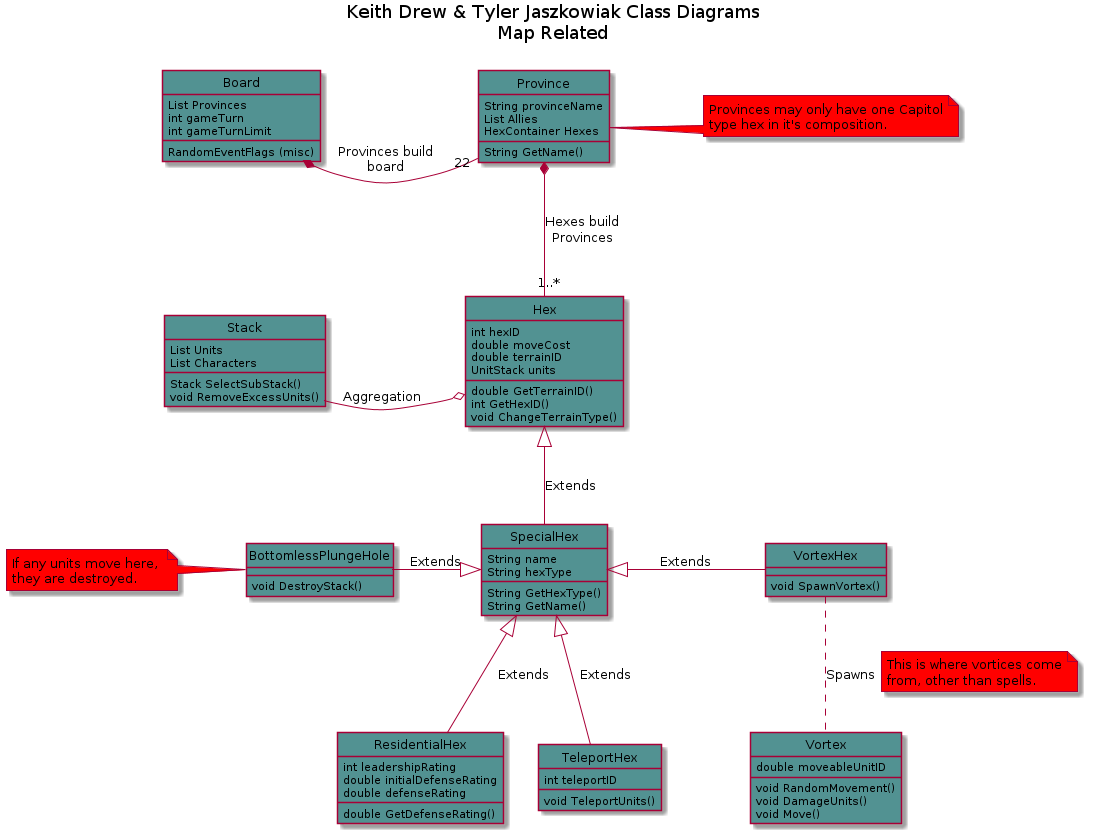
\includegraphics[width=\textwidth]{classD}
\subsubsection{PlantUML Source}
\begin{verbatim}
@startuml
title Keith Drew & Tyler Jaszkowiak Class Diagrams\nMap Related
hide circle
class Board #529292 {
      List Provinces
      RandomEventFlags (misc)
      int gameTurn
      int gameTurnLimit
}
class Province #529292 {
      String provinceName
      String GetName()
      List Allies
      HexContainer Hexes
}
note right of Province #red
     Provinces may only have one Capitol
     type hex in it's composition.
end note 
class Hex #529292 {
      int hexID
      double moveCost
      double terrainID
      UnitStack units
      double GetTerrainID()
      int GetHexID()
      void ChangeTerrainType()
}
class Stack #529292 {
      List Units
      List Characters
      Stack SelectSubStack()
      void RemoveExcessUnits()
}
class SpecialHex #529292 {
      String name
      String hexType
      String GetHexType()
      String GetName()
}
class ResidentialHex #529292 {
      int leadershipRating
      double initialDefenseRating
      double defenseRating
      double GetDefenseRating()
}
class BottomlessPlungeHole #529292 {
      void DestroyStack()
}
note left of BottomlessPlungeHole #red
     If any units move here, 
     they are destroyed.
end note 
class VortexHex #529292 {
      void SpawnVortex()
}
class TeleportHex #529292 {
      void TeleportUnits()
      int teleportID
}
class Vortex #529292 {
      double moveableUnitID
      void RandomMovement()
      void DamageUnits()
      void Move()
}
Board *-right- "22" Province : Provinces build\nboard 
Province *-down- "1..*" Hex : Hexes build\nProvinces
Hex <|-down- SpecialHex : Extends
Vortex .up. VortexHex : Spawns
note right on link #red
     This is where vortices come
     from, other than spells.
end note  
TeleportHex --up|> SpecialHex : Extends
VortexHex --left|> SpecialHex : Extends
BottomlessPlungeHole --right|> SpecialHex : Extends
ResidentialHex --up|> SpecialHex : Extends
Stack -lefto Hex : Aggregation
@enduml
\end{verbatim}

\section{Detail Diagrams}

\subsection{Blah Detail}

\section{PlantUML Source}

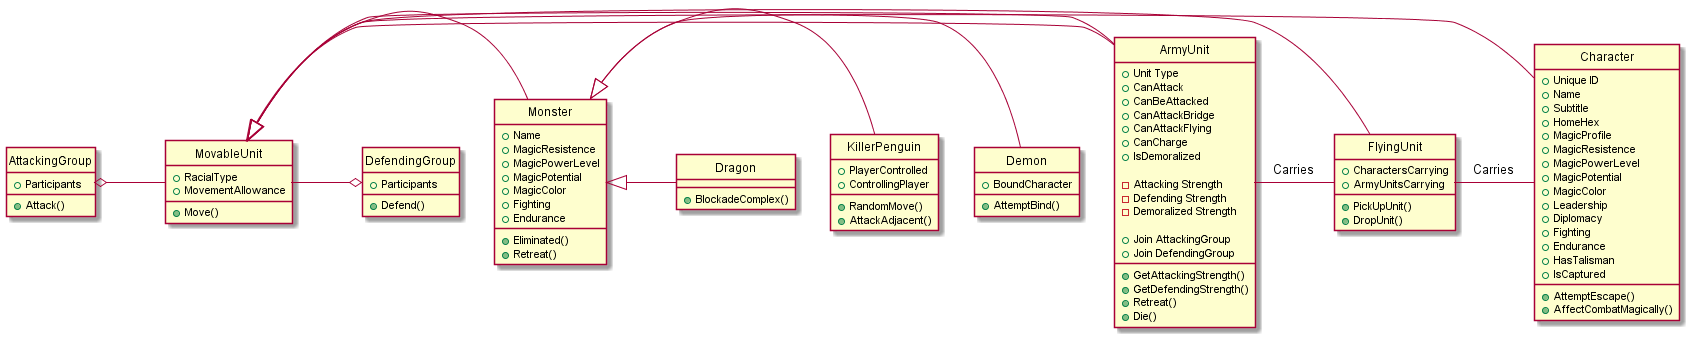
\includegraphics[width=\textwidth]{UnitDiagrams.png}

A movable unit is something with a race that a player can move.

An army unit is something that attacks and defends directly. Army
units are mostly differentiated by their fixed attacking and defending
strengths, and by restrictions on what sort of units and terrain they
can attack. Each individual army unit may be in several different
states. IsDemoralized is a state that can persist between game turns.
CanAttack and CanBeAttacked are states that are reset each game turn,
(these states stem from the rule that each unit can only participate
in a single attack each game turn).

What can an ArmyUnit do? Attack, defend, retreat and die. The games
rules are best reflected by considring attacking and defending as
group operations (possibly in a group of size 1). The AttackingGroup
and DefendingGroup classes capture this.

FlyingUnits are a subclass of normal ArmyUnits, but they can carry a
single unit or any number of characters.

\begin{verbatim}

@startuml
hide circle

MovableUnit <|- ArmyUnit
FlyingUnit -|> MovableUnit

FlyingUnit --  Character : Carries
ArmyUnit -- FlyingUnit : Carries

AttackingGroup o- MovableUnit
MovableUnit -o DefendingGroup

class AttackingGroup{
+ Participants
+ Attack()
}

class DefendingGroup{
+ Participants
+ Defend()
}

class ArmyUnit { 

+ Unit Type 
+ CanAttack
+ CanBeAttacked
+ CanAttackBridge
+ CanAttackFlying
+ CanCharge
+ IsDemoralized

- Attacking Strength
- Defending Strength
- Demoralized Strength

+ GetAttackingStrength()
+ GetDefendingStrength()
+ Join AttackingGroup
+ Join DefendingGroup
+ Retreat()
+ Die()

}


class FlyingUnit {
+ CharactersCarrying
+ ArmyUnitsCarrying
+ PickUpUnit()
+ DropUnit()
}

class MovableUnit {
+ RacialType
+ MovementAllowance
+ Move()
}


@enduml

\end{verbatim}

\end{document}
